\documentclass{article}

\usepackage{xcolor}
\definecolor{BLUELINK}{HTML}{0645AD}
\definecolor{DARKBLUELINK}{HTML}{0B0080}
\definecolor{LIGHTBLUELINK}{HTML}{3366BB}
\definecolor{PURPLELINK}{HTML}{663366}
\PassOptionsToPackage{hyphens}{url}
\usepackage[colorlinks=false ]{hyperref}
% for linking between references, figures, TOC, etc in the pdf document
\hypersetup{colorlinks,
linkcolor=DARKBLUELINK,
anchorcolor=DARKBLUELINK,
citecolor=DARKBLUELINK,
filecolor=DARKBLUELINK,
menucolor=DARKBLUELINK,
urlcolor=BLUELINK
} % Color citation links in purple
\PassOptionsToPackage{unicode}{hyperref}
\PassOptionsToPackage{naturalnames}{hyperref}

\usepackage{biorxiv} % github.com/alexsbaldwin/biorxiv-inspired-latex-style

\usepackage{url}
\usepackage{amssymb,amsfonts,amsmath,amsthm,mathtools}
\usepackage{textcomp}
\usepackage{gensymb}
\usepackage{cancel}
\usepackage{lmodern}
\usepackage{xfrac, nicefrac}
\usepackage{blkarray}
\usepackage{pgf,tikz}
\usetikzlibrary{positioning,arrows,automata,calc}
\usepackage{bm}
\usepackage{listings, enumerate, enumitem}
\usepackage[export]{adjustbox}
\usepackage{tabu}
\tabulinesep=0.6mm
\newcommand\cellwidth{\TX@col@width}
\usepackage{hhline}
\setlength{\arrayrulewidth}{1.2pt}
\usepackage{multicol,multirow,array}
\usepackage{etoolbox}
\AtBeginEnvironment{tabu}{\footnotesize}
\usepackage{booktabs}

\usepackage[flushleft] {threeparttable}
\usepackage{adjustbox}
\usepackage{bbold}
\usepackage{pdfpages}
\usetikzlibrary{positioning}
\usetikzlibrary{arrows,automata}
\pdfinclusioncopyfonts=1
\usepackage{nicefrac} % compact symbols for 1/2, etc.
\usepackage{microtype} % microtypography
\usepackage{lineno}

\graphicspath{{artworks/}}
\makeatletter
\def\input@path{{artworks/}}
\makeatother

\renewcommand{\baselinestretch}{1.5}

\definecolor{RED}{HTML}{EB6231}
\definecolor{YELLOW}{HTML}{E29D26}
\definecolor{BLUE}{HTML}{5D80B4}
\definecolor{LIGHTGREEN}{HTML}{6ABD9B}
\definecolor{GREEN}{HTML}{8FB03E}
\definecolor{PURPLE}{HTML}{BE1E2D}
\definecolor{BROWN}{HTML}{A97C50}
\definecolor{PINK}{HTML}{DA1C5C}

\newcommand{\der}{\mathrm{d}}
\newcommand{\e}{\mathrm{e}}
\newcommand{\dnds}{dNdS}
\newcommand{\indice}{l}
\newcommand{\indiceexp}{^{(\indice)}}
% Time, effective population size and mutation rate.
\newcommand{\Ne}{N}
% \acrshort{DNA}
\newcommand{\SetNuc}{\Omega_{\mathrm{N}}}
\newcommand{\SetWeak}{\Omega_{\mathrm{W}}}
\newcommand{\SetStrong}{\Omega_{\mathrm{S}}}
\newcommand{\mutmatrix}{R}
\newcommand{\Mutmatrix}{\bm{\mutmatrix}_{4\times4}}
\newcommand{\exchan}{\rho}
\newcommand{\Exchan}{\bm{\exchan}_{6\times1}}
\newcommand{\mutequi}{\sigma}
\newcommand{\Mutequi}{\bm{\mutequi}_{4\times1}}
% Codons
\newcommand{\SetCodon}{\Omega_{\mathrm{C}}}
\newcommand{\ci}{{i}}
\newcommand{\cj}{{j}}
\newcommand{\itoj}{\ci, \cj}
\newcommand{\nucitoj}{\mathcal{M}(\itoj)}
\newcommand{\submatrix}{Q}
\newcommand{\Submatrix}{\bm{\submatrix}_{61\times61}}
\newcommand{\subequi}{\pi}
\newcommand{\Subequi}{\bm{\subequi}_{61\times1}}
\newcommand{\probmatrix}{P}
\newcommand{\Probmatrix}{\bm{\probmatrix}_{61\times61}}
% Amino-acids
\newcommand{\SetAa}{\Omega_{\mathrm{A}}}
\newcommand{\Neighbor}{\mathcal{V}}
\newcommand{\NonSyn}{\mathcal{N}}
\newcommand{\Syn}{\mathcal{S}}
\newcommand{\Nx}{\Neighbor_x}
\newcommand{\NxAB}{\Neighbor_x^{\mathrm{A} \rightarrow \mathrm{B}}}
\newcommand{\NyBA}{\Neighbor_x^{\mathrm{B} \rightarrow \mathrm{A}}}
\newcommand{\NxWS}{\Neighbor_x^{\mathrm{W} \rightarrow \mathrm{S}}}
\newcommand{\NxSS}{\Neighbor_x^{\mathrm{S} \rightarrow \mathrm{S}}}
\newcommand{\NxSW}{\Neighbor_x^{\mathrm{S} \rightarrow \mathrm{W}}}
\newcommand{\NxWW}{\Neighbor_x^{\mathrm{W} \rightarrow \mathrm{W}}}
\newcommand{\NyWS}{\Neighbor_y^{\mathrm{W} \rightarrow \mathrm{S}}}
\newcommand{\NySS}{\Neighbor_y^{\mathrm{S} \rightarrow \mathrm{S}}}
\newcommand{\NySW}{\Neighbor_y^{\mathrm{S} \rightarrow \mathrm{W}}}
\newcommand{\NyWW}{\Neighbor_y^{\mathrm{W} \rightarrow \mathrm{W}}}
\newcommand{\NxNonSyn}{\NonSyn_x}
\newcommand{\NyNonSyn}{\NonSyn_y}
\newcommand{\NxSyn}{\Syn_x}
\newcommand{\NySyn}{\Syn_y}
\newcommand{\aminoacid}{\text{A}}
\newcommand{\aai}{\mathcal{A}(\ci)}
\newcommand{\aaj}{\mathcal{A}(\cj)}
\newcommand{\Ni}{\mathcal{N}_{\mathrm{eighbors}}\left(\ci\right)}
\newcommand{\NiNonSyn}{\mathcal{N}_{\mathrm{onSyn}}\left(\ci\right)}
\newcommand{\NiSyn}{\mathcal{S}_{\mathrm{yn}}\left(\ci\right)}
\newcommand{\fit}{f}
\newcommand{\Fit}{\bm{\fit}_{20\times1}}
\newcommand{\fiti}{\fit_{\aai}}
\newcommand{\fitj}{\fit_{\aaj}}
\newcommand{\scaledfit}{F}
\newcommand{\ScaledFit}{\bm{\scaledfit}_{20\times1}}
\newcommand{\scaledfiti}{\scaledfit_{\aai}}
\newcommand{\scaledfitj}{\scaledfit_{\aaj}}
\newcommand{\selcoef}{{\delta_{\fit}}}
\newcommand{\scaledselcoef}{{\Delta \scaledfit}}
% Tree
\newcommand{\Tree}{\mathcal{T}}
\newcommand{\node}{\text{v}}
\newcommand{\taxon}{\node}
\newcommand{\Settaxon}{1 \leq \taxon \leq \Ntaxa}
\newcommand{\Ntaxa}{P}
\newcommand{\treeroot}{0}
\newcommand{\treerootexp}{^{(\treeroot)}}
\newcommand{\branch}{\text{w}}
\newcommand{\branchexp}{^{(\branch)}}
\newcommand{\Nbranch}{2 \Ntaxa - 2}
\newcommand{\Setbranch}{1 \leq \branch \leq 2 \Ntaxa - 2}
\newcommand{\up}{\branch^{\uparrow}}
\newcommand{\down}{\node}
\newcommand{\nodeexp}{^{(\node)}}
\newcommand{\Nnode}{2 \Ntaxa - 2}
\newcommand{\Ninternal}{\Ntaxa - 2}
\newcommand{\Setnode}{\treeroot \leq \node \leq 2 \Ntaxa - 2}
\newcommand{\Setnodenoroot}{1 \leq \node \leq 2 \Ntaxa - 2}
\newcommand{\Setinternal}{\Ntaxa + 1 \leq \node \leq 2 \Ntaxa - 2}
\newcommand{\branchnode}{\mathcal{W}}
\newcommand{\age}{T}
\newcommand{\branchtime}{\Delta \age}
\newcommand{\branchlength}{L}
% Alignment
\newcommand{\data}{{\color{PINK}{D}}}
\newcommand{\Data}{\bm{\data}}
\newcommand{\site}{\text{s}}
\newcommand{\siteexp}{^{(\site)}}
\newcommand{\Nsite}{\text{N}_{\site}}
\newcommand{\Setsite}{1 \leq \site \leq \Nsite}
\newcommand{\branchsiteexp}{^{(\branch, \site)}}
\newcommand{\treerootsiteexp}{^{(\treeroot, \site)}}
\newcommand{\taxonsiteexp}{^{(\taxon, \site)}}
% Categories
\newcommand{\cat}{\text{k}}
\newcommand{\catVar}{\mathcal{K}}
\newcommand{\catexp}{^{(\cat)}}
\newcommand{\Ncat}{\text{N}_{\cat}}
\newcommand{\Setcat}{1 \leq \cat \leq \Ncat}
\newcommand{\catsite}{\catVar^{\left(\site\right)}}
\newcommand{\branchcatexp}{^{(\branch, \cat)}}
\newcommand{\treerootcatexp}{^{(\treeroot, \cat)}}
% Polymorphism
\newcommand{\copies}{\text{n}}
\newcommand{\samples}{\text{N}_{\copies}}
% Random variables
\newcommand{\pruning}{\psi}
\newcommand{\uniform}{0, 1}
\newcommand{\Identitymatrix}{\bm{I}_{2\times2}}
\newcommand{\brownian}{\bm{B}_{2\times1}}
\newcommand{\contrast}{\bm{C}_{2\times1}}
\newcommand{\Covariancematrix}{\bm{\varSigma}_{2\times2}}
\newcommand{\covariancedf}{q}
\newcommand{\covariancekappa}{\kappa}
\newcommand{\Scattermatrix}{\bm{A}_{2\times2}}
\newcommand{\Multivariate}{\bm{Z}_{2\times1}}
\newcommand{\base}{\varPi}
\newcommand{\Base}{\bm{\base}_{20\times1}}
\newcommand{\baseconc}{\alpha}
\newcommand{\Basecenter}{\bm{\gamma}_{20\times1}}
\newcommand{\stickbreaking}{\varOmega}
\newcommand{\StickBreaking}{\bm{\stickbreaking}_{\Ncat\times1}}
\newcommand{\stick}{\varPhi}
\newcommand{\stickbreakinghyper}{\beta}
% Mapping
\newcommand{\history}{\mathcal{H}}
\newcommand{\sn}{{\color{BLUE}{S}}}
\newcommand{\s}{{\color{LIGHTGREEN}{S_0^{k}}}}
\newcommand{\si}{{\color{PINK}{S_1^{k}}}}
\newcommand{\sii}{{\color{PINK}{S_2^{k}}}}
\newcommand{\siii}{{\color{PINK}{S_3^{k}}}}
\newcommand{\siiii}{{\color{PINK}{S_4^{k}}}}
\newcommand{\siiiii}{{\color{LIGHTGREEN}{S_5^{k}}}}


\linenumbers

\title{Robustness of codon models to mutational bias}

%\date{September 9, 1985}	% Here you can change the date presented in the paper title
%\date{} 					% Or removing it

\author{
 \large
 T. {Latrille}$^{1,2}$, N. {Lartillot}$^{1}$ \\
 \normalsize
	$^{1}$Université de Lyon, Université Lyon 1, CNRS, Laboratoire de Biométrie et Biologie Évolutive UMR 5558, F-69622 Villeurbanne, France.\\
	$^{2}$École Normale Supérieure de Lyon, Université de Lyon, Université Lyon 1, Lyon, France\\
	\texttt{\href{mailto:thibault.latrille@ens-lyon.org}{thibault.latrille@ens-lyon.org}} \\
}

% Uncomment to override the `A preprint' in the header
%\renewcommand{\headeright}{}

\begin{document}
\maketitle

\begin{abstract}
 Nucleotide composition in protein-coding sequences is the result of the equilibrium between mutation and selection.
 Because of selection, the nucleotide composition of protein-coding sequences is different from what would be expected under a pure mutational process.
 In particular, it differs between the three coding positions, with the third position showing more extreme composition than the first and the second positions.
 This empirical observation is well known, yet, phylogenetic codon models do not correctly capture this phenomenon.
 Instead, in their classical parameterization, in terms of a 4x4 nucleotide rate matrix and a single $\omega$ parameter, phylogenetic codon models predict that the nucleotide composition should be the same for all $3$ positions of the codons, and should be equal to the equilibrium frequencies of the underlying 4x4 nucleotide process.
 Alternatively, to accommodate this variation across coding positions, some models allow for different nucleotide rate matrices at the three positions.
 However, this approach is problematic since the mutation process should in principle be blind to the coding structure, and should be homogeneous across coding positions.
 Although this misconception has probably minor impact on the detection of positive selection, it is a clear symptom of a more fundamental issue with teasing apart mutation rates and fixation biases in phylogenetic codon models.
 Practically, this could have important consequences, in particular, given the current interest in modelling the impact of GC-biased gene conversion ({gBGC}) on the evolution of protein-coding sequences, a factor which requires mutation and fixation biases to be carefully disentangled.
 Conceptually, the problem comes from the fact that, at the mutation-selection equilibrium, there is a net selection differential, or net fixation bias, acting against the mutational pressure.
 In other words, at equilibrium, $\omega$ is not the same in different mutational directions.
 Because they capture selection through a single parameter $\omega$, phylogenetic codon models cannot correctly capture this net fixation bias.
 To address this problem, we present an alternative modelling approach, where $\omega$ is not seen as a scalar anymore, but as a tensor of $\omega$ values unfolding along multiple directions.
 This tensor captures the small differences in fixation rate (or $\omega$) in different directions, which gives an accurate representation of how mutation and selection oppose each other at equilibrium.
 This parameterization is the simplest one, in a phenomenological context, capable of correctly teasing apart mutation and selection.
 Thanks to this, this modelling approach yields a reliable estimate of the mutational process, while disentangling fixation probabilities in different directions.
\end{abstract}

% keywords can be removed
\keywords{codon models \and phylogenetics \and nucleotide bias \and mutation-selection models.}

\section{Introduction}

%%Introducing codon models and their usefulness
Phylogenetic codon models are now routinely used in many domains of bioinformatics and molecular evolutionary studies.
One of their main applications has been to characterize the genes, sites~\citep{Nielsen1998}, or lineages~\citep{Zhang2004} having experienced positive selection.
More generally, these models highlight the respective contributions of mutation, selection, {genetic drift} and biased gene conversion~\citep{Kosiol2019}, and the causes of their variation between genes~\citep{Zhang2015} or across species~\citep{Lartillot2011}.

%introducing the idea of a single $\omega$
Conceptually, codon models take advantage of the fact that {synonymous} and {non-synonymous} {substitutions} are differentially impacted by selection.
Assuming {synonymous} mutations are {neutral}, the {synonymous} {substitution} rate is equal to the underlying mutation rate~\citep{kimura1983neutral}.
Non-synonymous {substitutions}, on the other hand, reflect the combined effect of mutation and selection~\citep{Ohta1995}.
Classical codon models formalize this idea by invoking a single parameter $\omega$, acting multiplicatively on {non-synonymous} {substitutions} rates~\citep{Muse1994, Goldman1994}.
Using a parametric model automatically corrects for the multiplicity issues created by the complex structure of the genetic code and by uneven mutation rates between nucleotides.
As a result, $\omega$ captures the net, or aggregate, effect of selection on {non-synonymous} mutations (also called $\dnds$).

%elaborating on the phenomenological versus mechanistic, classical versus mutsel, distinction
Classical codon models, so defined, are phenomenological, in the sense that they capture a complex mixture of selective effects through a single parameter~\citep{Rodrigue2010a}.
In reality, the selective effects associated with {non-synonymous} mutations depends on the context (site-specificity) and the amino acids involved in the transition~\citep{Kosiol2007}.
Attempts at an explicit modelling of these complex selective landscapes have also been done, leading to mechanistic codon models, based on the mutation-selection formalism~\citep{Halpern1998}.
These models, further developed in multiple inference frameworks~\citep{Rodrigue2010, Tamuri2012}, sometimes using empirically informed fitness landscapes~\citep{Bloom2014}, could have many interesting applications, such as inferring the distribution of fitness effects~\citep{Tamuri2012} or detecting genes under adaptation~\citep{Rodrigue2016}, or even phylogenetic inference.
However, they are computationally complex and potentially sensitive to the violation of their assumptions about the fitness landscape (such as site independence).
For this reason, phenomenological codon models remain an attractive, potentially more robust, although still perfectible approach.

%bringing in the key issue here: correctly teasing apart mutation and selection
The parametric design of typical codon models, relying on a single aggregate parameter $\omega$, raises the question whether they reliably estimate the underlying mutational process.
Several observations suggest that this may not be the case.
For instance, in their simplest form~\citep{Muse1994, Goldman1994}, codon models predict that the nucleotide composition should be the same for all three positions of the codons, and should be equal to the nucleotide equilibrium frequencies implied by the underlying nucleotide {substitution} rate matrix.
In reality, the nucleotide composition differs: the third position shows more extreme GC composition, reflecting the underlying mutation bias, compared to the first and second positions, which are typically closer to 50\% GC~\citep{Singer2000}.

These modulations across the three coding positions have been accommodated using the so-called 3x4 formalism~\citep{Goldman1994, Pond2005a}, allowing for different nucleotide rate matrices at the three coding positions.
However, this is also problematic, since this modelling approach has the consequence that {synonymous} {substitutions}, say, from A to C, occur at different rates at the first and third positions.
Yet, in reality, the mutation process is blind to the coding structure, and should be homogeneous across coding positions, and if {neutral}, all mutations from A to C should thus have the same rate.

%Potential impact of these problems: both practical and conceptual
These observations suggest that the mutation matrix (1x4) or matrices (3x4) estimated by codon models are not correctly reflecting the mutation rates between nucleotides~\citep{Rodrigue2008a}.
Instead, what these matrices are capturing is the result of the compromise between mutation and selection at the level of the realized nucleotide frequencies.
For detecting selection, this problem is probably minor, although it still bears consequences on the estimation of $\omega$~\citep{Spielman2015}.
Conceptually, however, it is a clear symptom of a more fundamental problem: mutation rates and fixation probabilities are not correctly teased apart by current codon models.

Practically, this misconception could have important consequences in contexts other than tests of positive selection.
In particular, there is a current interest in investigating the variation between species in GC content, and its effect on the evolution of protein-coding sequences~\citep{Bolivar2019}.
An important factor here is biased gene conversion toward GC (called {gBGC}), which can confound the tests for detecting positive selection and, more generally, the estimation of $\omega$~\citep{Galtier2009,Ratnakumar2010, Figuet2014}.
Even in the absence of {gBGC}, however, uneven mutation rates varying across species can have an important impact on the estimation of the strength of selection.
All this suggests that, even before introducing {gBGC} in codon models, correctly formalizing the interplay between mutation and selection in current codon models would be an important first step.

%The mut-sel balance revisited: an equilibrium between two net forces
In this direction, the key point that needs to be correctly formalized is the following.
If the nucleotide's realized frequencies are the result of a compromise between mutation and selection, then this implies that the strength of selection is not the same between all nucleotide or amino-acid pairs.
For instance, if the mutation process is AT-biased, then, because of selection, the realized nucleotide frequencies at equilibrium will be less AT-biased than expected under the pure mutation process.
However, this implies that, at equilibrium, there will be a net mutation pressure toward AT, which has to be compensated for by a net selection differential toward GC.

%introducing $\omega$ as a tensor
All this suggests that, in order for a codon model to correctly formalize this subtle interplay between mutation and selection, the component of the parameter vector responsible for absorbing the net effect of selection (i.e.~$\omega$) should not be a scalar, as is currently the case.
Instead, it should be a tensor, that is, an array of $\omega$ values unfolding along multiple directions.
In the present work, we address the question of whether we can derive a parametric structure being able correctly tease apart mutation rates and selection, and this, without having to explicitly model the underlying fitness landscape.
In order to derive a codon model along those lines, our strategy is to first assume a true site-specific evolutionary process, following the mutation-selection formalism.
Then, we derive the mean {substitution} process implied across all sites by this mechanistic model and identify the mean fixation probabilities appearing in this mean-field process with the $\omega$ tensor to be estimated.
Inferring parameters on simulated alignments, we show that the model correctly estimates the mutation rates, as well as the mean effect of selection.

\section{Results}
\label{sec:results}

To illustrate the problem, we first conduct simulation experiments under a simple mutation-selection {substitution} model assuming site-specific amino-acid preferences.
We use these simulation experiments to explore through summary statistics the intricate interplay between mutation and selection.
Then, we explore how codon models with different parameterizations are able to infer the mutation rates and the strength of selection on these simulated alignments.
Finally, these alternative models are applied to empirical data.

\subsection{Simulations experiments}
\label{subsec:simulations-experiments}

Simulations of protein-coding {DNA} sequences were conducted under an origination-fixation {substitution} process~\citep{McCandlish2014} at the level of codons (see section~\ref{sec:mut-bias-simu}).
We assume a simple mutation process with a single parameter controlling the mutational bias toward AT, denoted $\lambda = (\mutequi_A+\mutequi_T)/(\mutequi_C+\mutequi_G)$, where $\mutequi_x$ is the equilibrium frequency of nucleotide $x$.
This mutational process is shared by all sites of the sequence.
With regards to selection, {synonymous} mutations are considered {neutral}, such that the {synonymous} {substitution} rate equal to the underlying mutation rate.
At the protein level, selection is modelled by introducing site-specific amino-acid fitness profiles (i.e.~a vector of 20 fitnesses for each coding site), which are scale by a relative effective population size $\Ner$.
A high $\Ner$ induces site-specific profiles having a large variance, with some amino acids with a high scaled fitness while all other have a low scaled fitness.
Conversely, a low value for $\Ner$ induces more even amino-acid fitness profiles (i.e.~neutral) at each site.
Thus, ultimately, the stringency of selection increase with $\Ner$.
Altogether, the two parameters of the model tune the mutation bias ($\lambda$) and the stringency of selection ($\Ner$), respectively.

All simulations presented are obtained using the same underlying tree topology and branch length of 61 primates from \citet{Perelman2011}, and 4980 codon sites with amino-acid fitness profiles resampled from experimentally determined profiles in \citet{Bloom2017}.
Simulation of this origination-fixation process along a species tree result in a multiple sequence alignment of coding sequences for the extant species, from which summary statistics can then be computed.
One such straightforward summary statistic is the frequency of the different nucleotides, and the resulting nucleotide bias $\atgc$ observed in the alignment.
This observed nucleotide bias can be computed separately for each coding position (first, second and third) and compared to the underlying true mutational bias $\lambda$.
As can be seen from figure~\ref{fig:simu-mut-bias}, the third position of codons (panel C) reflects the underlying mutational bias quite faithfully, while the first and second positions (panel A and B) are impacted by the strength of selection and display nucleotide biases that are less extreme than the one implied by the mutational process.
This differential effect across the three coding positions is explained by nucleotide mutations at the third codon position being more often {synonymous}, while mutations at the first and second positions are more often changing the amino-acid and are thus more often under purifying selection.

\begin{figure}[h]
 \centering
 \begin{minipage}{0.32\linewidth}
 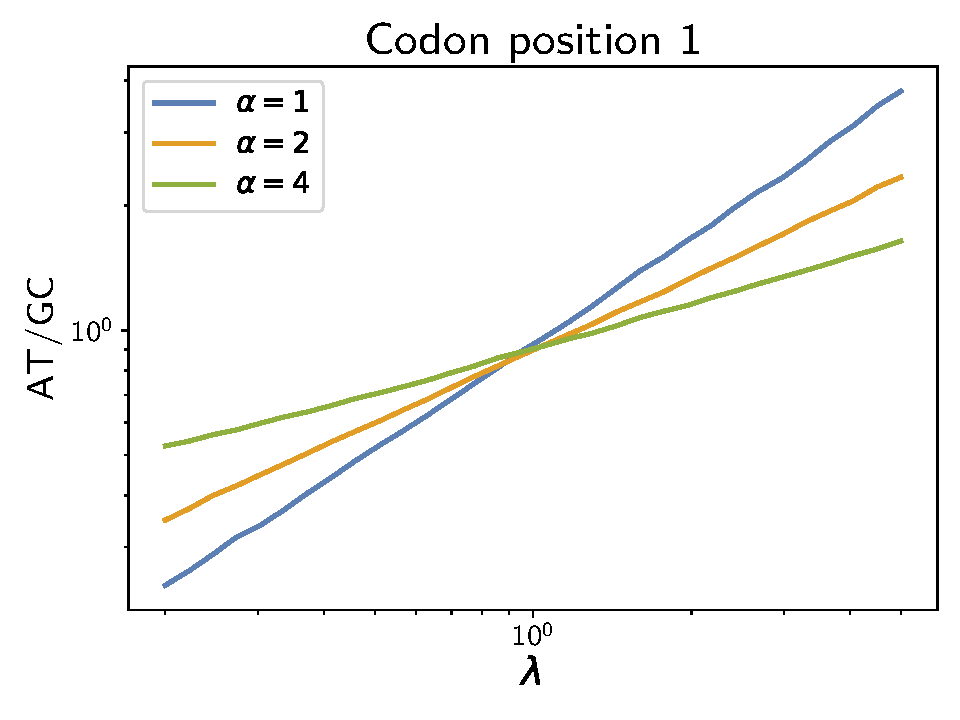
\includegraphics[width=\linewidth, page=1]{simulations/at_over_gc_1}
 \end{minipage}
 \llap{\raisebox{1.25cm}{\scriptsize A\hspace{4.15cm}}}\hfill
 \begin{minipage}{0.32\linewidth}
 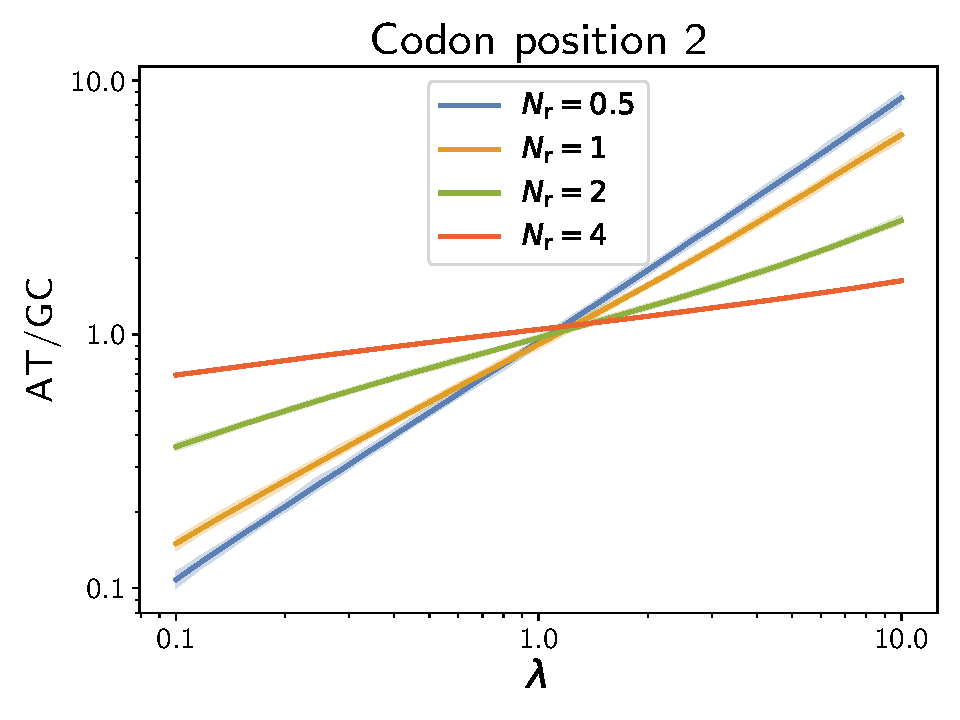
\includegraphics[width=\linewidth, page=1]{simulations/at_over_gc_2}
 \end{minipage}
 \llap{\raisebox{1.25cm}{\scriptsize B\hspace{4.15cm}}}\hfill
 \begin{minipage}{0.32\linewidth}
 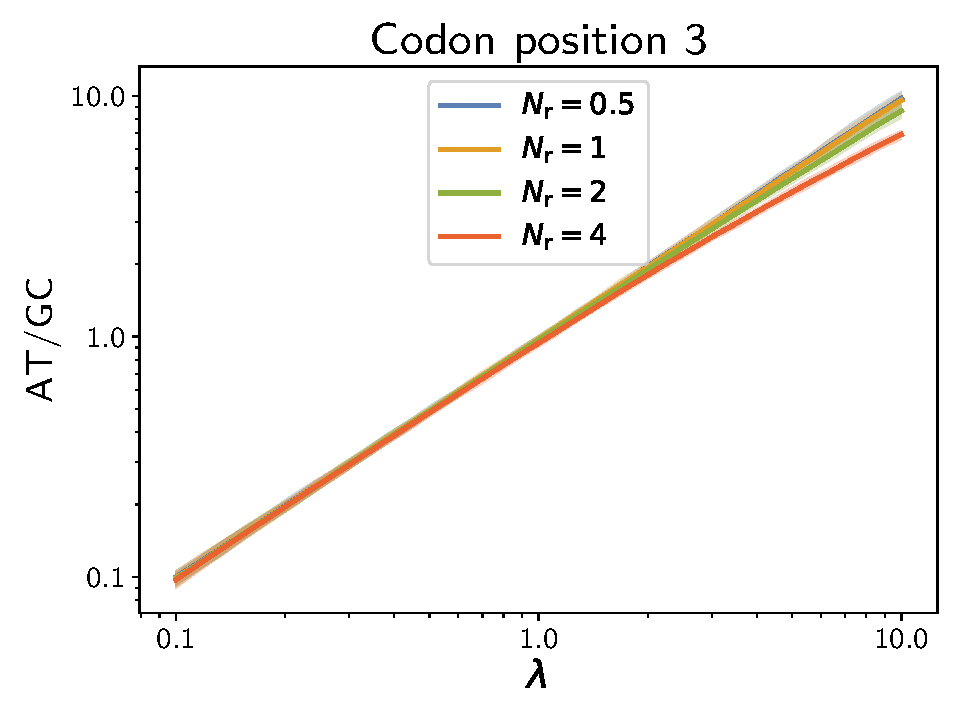
\includegraphics[width=\linewidth, page=1]{simulations/at_over_gc_3}
 \end{minipage}
 \llap{\raisebox{1.25cm}{\scriptsize C\hspace{4.15cm}}}\hfill
 \begin{minipage}{0.32\linewidth}
 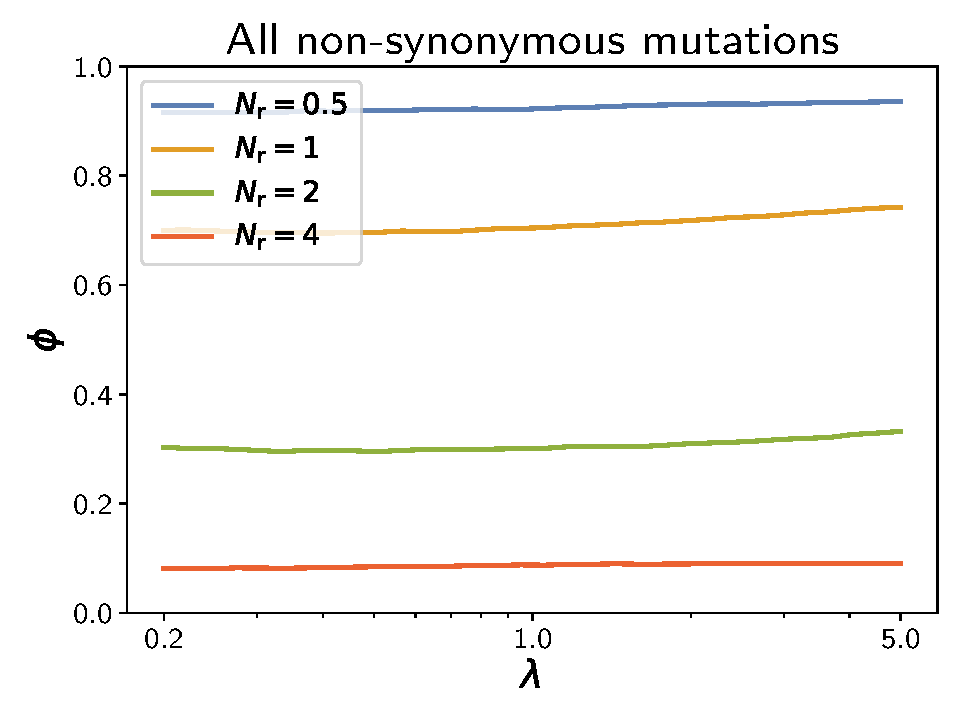
\includegraphics[width=\linewidth, page=1]{simulations/omega}
 \end{minipage}
 \llap{\raisebox{1.15cm}{\scriptsize D\hspace{4.15cm}}}\hfill
 \begin{minipage}{0.32\linewidth}
 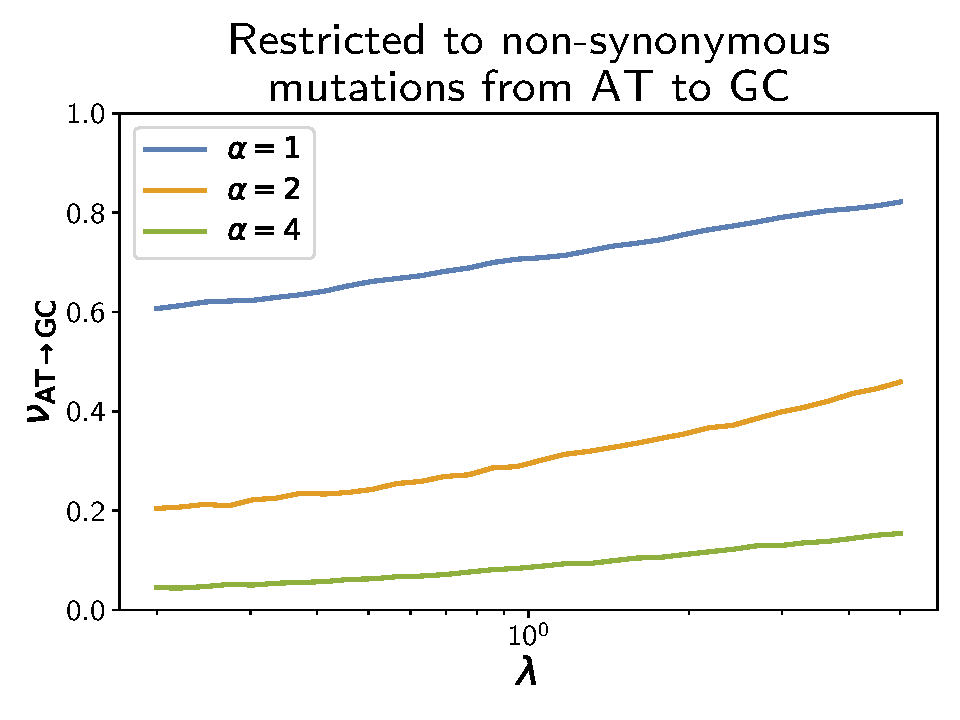
\includegraphics[width=\linewidth, page=1]{simulations/omega_WS}
 \end{minipage}
 \llap{\raisebox{0.80cm}{\scriptsize E\hspace{4.15cm}}}\hfill
 \begin{minipage}{0.32\linewidth}
 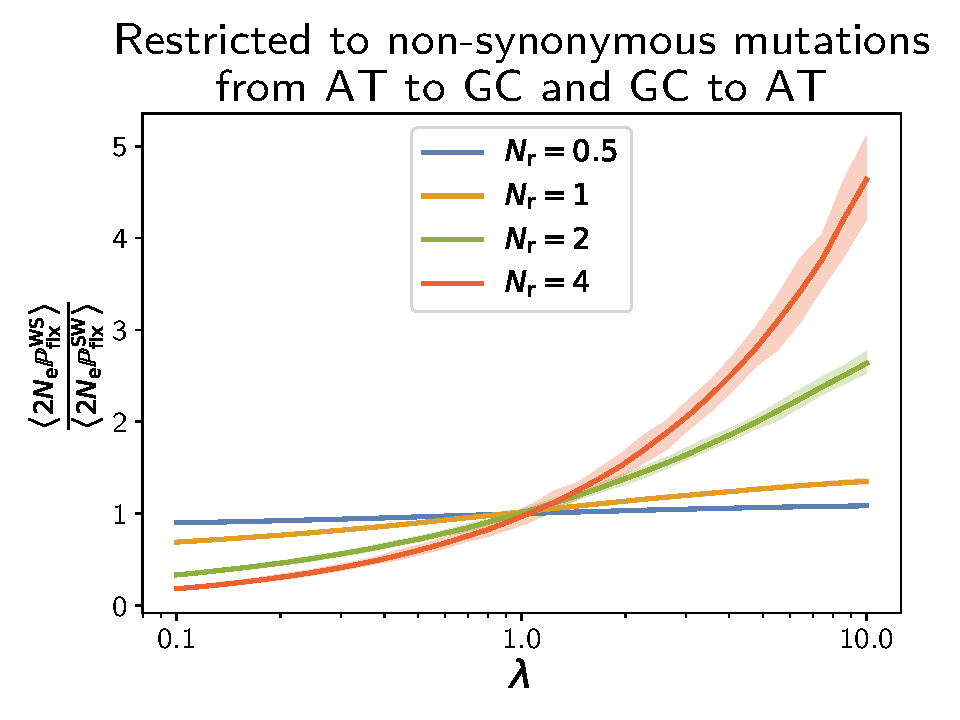
\includegraphics[width=\linewidth, page=1]{simulations/omega_WS_over_SW}
 \end{minipage}
 \llap{\raisebox{0.80cm}{\scriptsize F\hspace{4.15cm}}}\hfill
 \caption[$\atgc$ composition of the alignment]{
 Simulations of 61 primates taxa, 4980 codon sites, with 100 repeats. Solid lines represent the mean value over the repeats, and the colored area the 95\% inter-quantile range.
 Top row:
 Observed $\atgc$ composition of simulated alignment summed over all sites in vertical axis, represented at the different positions of codons (first, second and third), as a function the underlying mutational bias toward AT of the nucleotide matrix~($\lambda$).
 Stringency of selection (i.e. the relative effective population size $\Ner$) is represented by 4 coloured solid lines.
 $\atgc$ at the third codon position (panel C) matches the mutational bias, whereas in contrast first and second positions (panel A and B) are less extreme than the underlying bias.
 With decreased stringency of selection, the observed $\atgc$ is more tightly reflecting the underlying mutational bias.
 Bottom row: Mean scaled fixation probability of non-synonymous mutations along simulations, $\avgpfix$, as a function of mutational bias ($\lambda$), for different stringency of selection ($\Ner$).
 In panel D, expectedly, $\avgpfix$ decrease with increased $\Ner$ while is relatively unaffected by the mutational bias ($\lambda$).
 In panel E, $\avgpfixATtoGC$ is restricted to mutations from weak nucleotides (AT) to strong nucleotides (GC), where an AT-biased mutational process leads to an increased fixation probability toward GG.
 In panel F, $\avgpfixATtoGC$ is normalized by the fixation probabilities in the opposing direction $\avgpfixGCtoAT$, increasing monotonously with $\lambda$.
 Altogether, mutational bias is balanced by selection in the opposite direction, where this effect increases with the stringency of selection.
 }
 \label{fig:simu-mut-bias}
\end{figure}

Apart from the observed nucleotide bias in the alignment, a statistic directly relevant for measuring the intrinsic effect of selection is the mean scaled fixation probability of {non-synonymous} mutations, called $\avgpfix$.
This summary statistic $\avgpfix$ can be quantified from the {substitutions} recorded along the simulation trajectory (see section~\ref{subsec:fixation-bias}).
For very long trajectories, it identifies with the ratio of {non-synonymous} over {synonymous} {substitution} rates (or $\dnds$) induced by the underlying mutation-selection model~\citep{Spielman2015, DosReis2015, Jones2016}.
As expected, $\avgpfix$ is always lower than 1 for simulations at equilibrium, under a time-independent fitness landscape~\citep{Spielman2015}.
Quite expectedly $\avgpfix$ depends strongly on the stringency of selection ($\Ner$), which it is meant to measure~(figure~\ref{fig:simu-mut-bias}, panel D).
On the other hand, $\avgpfix$ depends weakly on the mutational bias ($\lambda$).

The proxy of selection represented by $\avgpfix$ concerns all {non-synonymous} mutations, but we can also consider the mean scaled fixation probability only for the subset of {non-synonymous} mutations from weak nucleotides (A or T) to strong nucleotides (G or C), called $\avgpfixATtoGC$.
Interestingly, $\avgpfixATtoGC$ increases with the strength of the mutational bias toward AT~(figure~\ref{fig:simu-mut-bias}, panel E).
This distortion of the selective effects toward GC is stronger under an increased stringency of selection, under a higher $\Ner$.
Likewise, the {non-synonymous} mutations could also be restricted from strong (GC) to weak nucleotides (AT).
This ratio decreases with the strength of the mutational bias toward AT (not shown).
As a result, the ratio ratio between $\avgpfixATtoGC$ and $\avgpfixATtoGC$ is higher than 1 under an mutational bias toward AT (and lower than 1 respectively for a bias toward GC).
It is monotonously increasing with the mutational bias toward AT~(figure~\ref{fig:simu-mut-bias}, panel F).
Altogether, fixation probabilities are opposed to mutational bias, and the realized equilibrium frequencies are thus at an equilibrium point between these two opposing forces.

\subsection{Parameter inference on simulated data}
\label{subsec:parameter-inference-on-simulated-data}

From an alignment of protein-coding {DNA} sequences, without knowing the specific history of {substitutions}, can one estimate the mutational bias ($\lambda$) and the mean scaled fixation probability $\avgpfix$?
In other words, can we tease apart mutation and selection?

To address this question, here we consider two codon models for inference, differing only by their parametrization of the codon matrix $\Submatrix$.
Both are homogeneous along the sequence (i.e.~not site-specific).
The first is based on \citet{Muse1994} formalism and uses a scalar $\omega$ parameter, while the second is based on a tensor representation of $\omega$.

\begin{figure}[!htb]
 \centering
 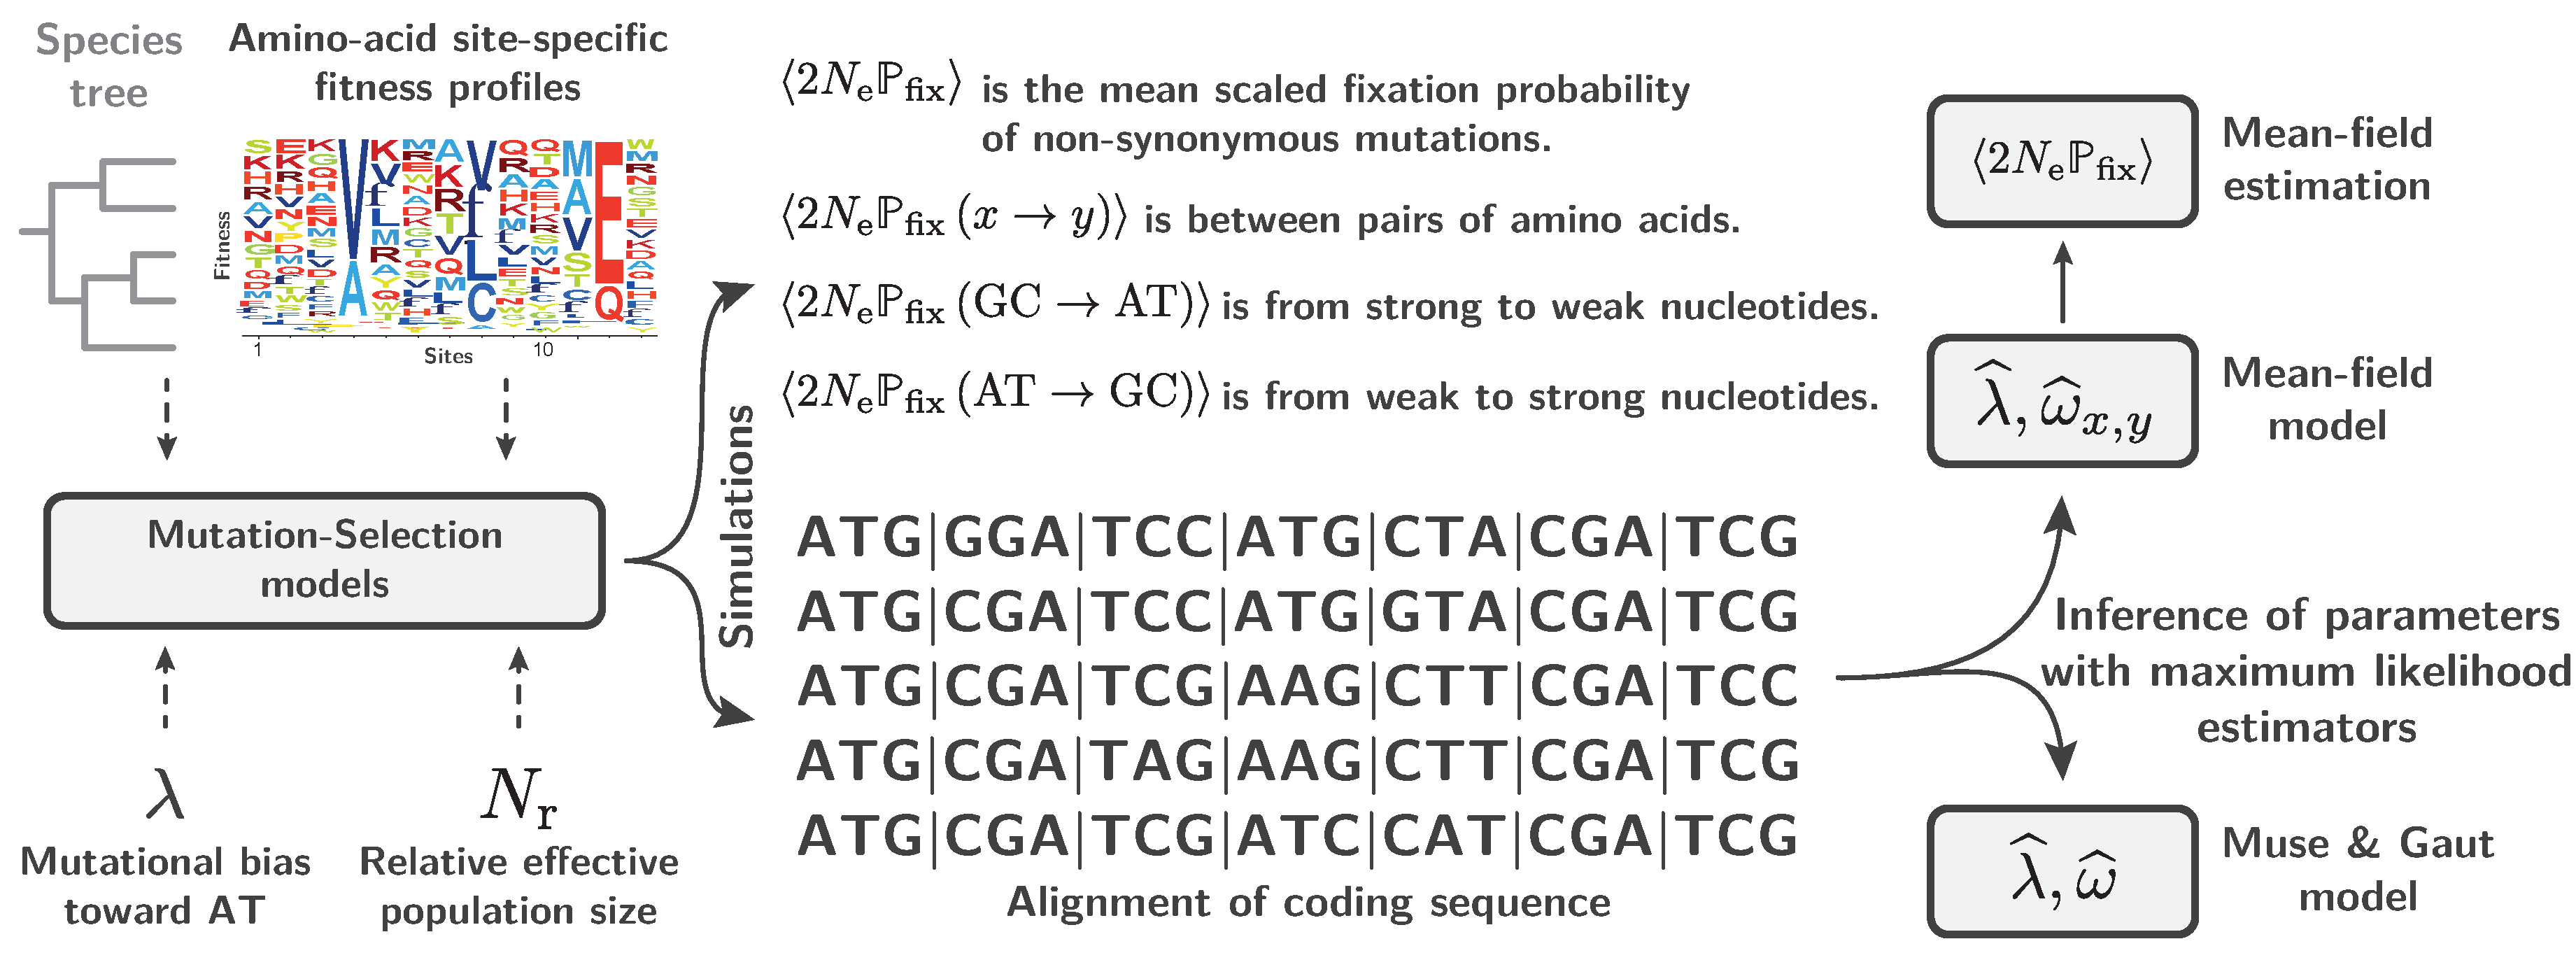
\includegraphics[width=\textwidth, page=1] {pipeline}
 \begin{minipage}{0.325\linewidth}
 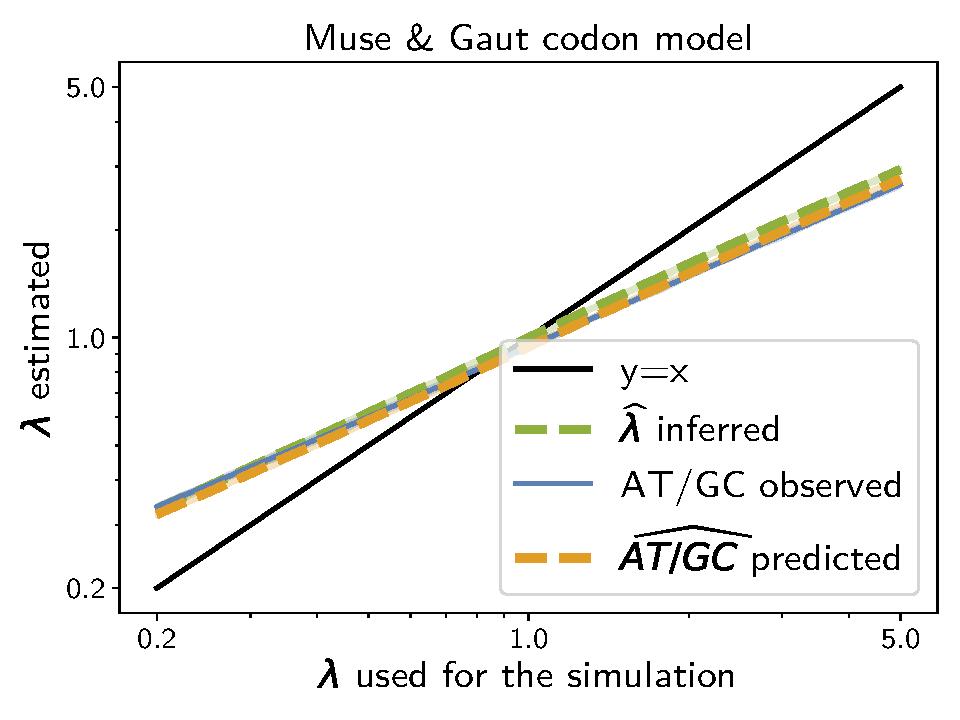
\includegraphics[width=\linewidth, page=1]{inference_simulations/lambda_MG}
 \end{minipage}
 \llap{\raisebox{1.25cm}{\scriptsize A\hspace{4.35cm}}}\hfill
 \begin{minipage}{0.325\linewidth}
 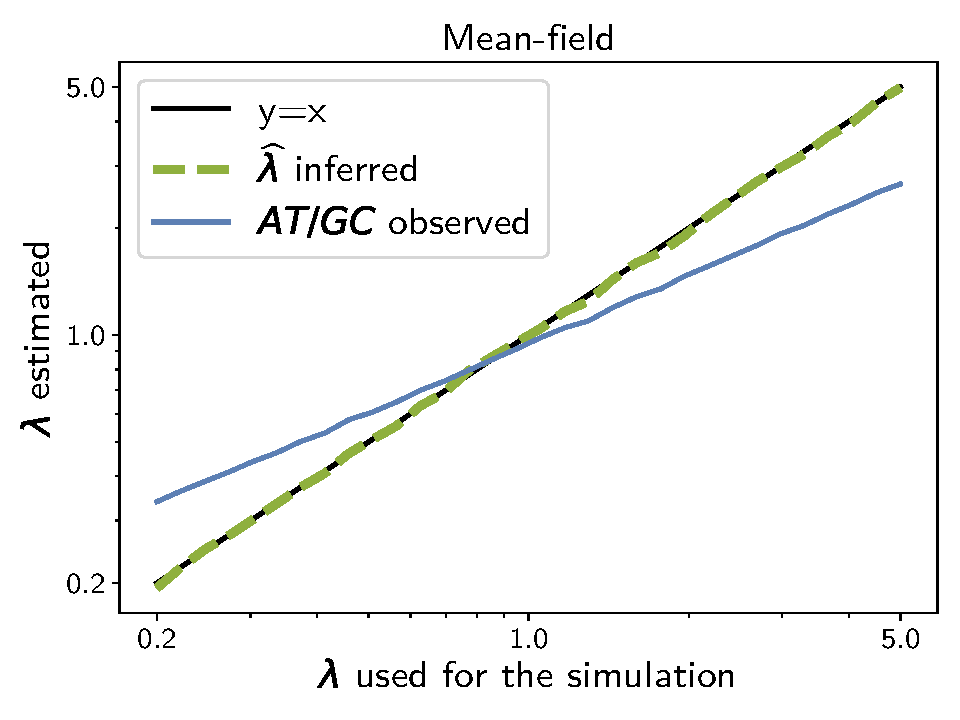
\includegraphics[width=\linewidth, page=1]{inference_simulations/lambda_MF}
 \end{minipage}
 \llap{\raisebox{1.25cm}{\scriptsize B\hspace{4.35cm}}}\hfill
 \begin{minipage}{0.325\linewidth}
 	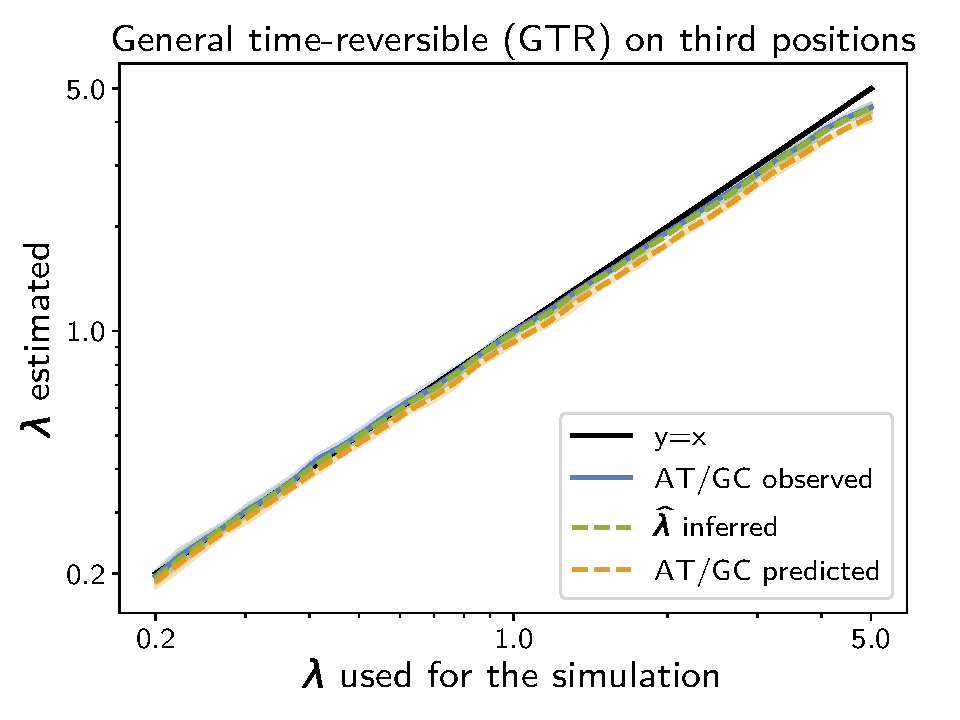
\includegraphics[width=\linewidth, page=1]{inference_simulations/lambda_GTR}
 \end{minipage}
 \llap{\raisebox{1.25cm}{\scriptsize C\hspace{4.35cm}}}\hfill
 \caption[Estimation of mutational bias]{
 The main goal is to derive a model of inference that can reliably estimate parameters of mutation and selection on simulated alignments (61 primates taxa, 4980 codon sites).
 Selection is modelled as a single $\omega$ parameter in the Muse \& Gaut formalism ({MG}) in panel A, while selection is modelled as a tensor of $\omega$ parameters between pairs of amino acids using a mean-field ({MF}) approximation in panel B.
 Different estimates of the mutational bias in vertical axis are represented as a function of the underlying true mutational bias ($\lambda$) during the simulation in horizontal axis.
 The estimated mutational bias $\widehat{\lambda}_{\text{{MG}}}$ (in green dotted line) in the {MG} formalism is between the true value (black solid line) and the observed $\atgc$ (blue solid line).
 Conversely, estimated mutational bias $\widehat{\lambda}_{\text{{MF}}}$ in the {MF} approximation equals to the underlying value.
 Finally, a general time-reversible model (panel C) can be applied to the third positions of codon (4-fold degenerated), which estimates reliably the underlying mutational bias.
 Altogether, the {MF} approximation can tease apart mutation and selection, while the {MG} formalism has to reach a compromise between observed $\atgc$ and underlying mutational bias.
 }
 \label{fig:mut-bias-inference}
\end{figure}

\subsubsection{\texorpdfstring{$\omega$}{ω} as a scalar: the Muse \& Gaut formalism}
This model is defined in terms of a generalized time-reversible nucleotide rate matrix $\Mutmatrix$ and a scalar parameter $\omega$.
The matrix $\Mutmatrix$ is a function of the nucleotide frequencies $\Mutequi$ and the symmetric exchangeability rates $\Exchan$~\citep{Tavare1986}:
\begin{equation}
 \mutmatrix_{a, b} = \exchan_{a,b}\mutequi_b
\end{equation}
At the level of codons, the {substitution} rate between the source ($\ci$) and target codon ($\cj$) depends on the underlying nucleotide change between the codons $\nucitoj$~(e.g.~$\nuc(AAT, AAG) = TG$), and whether or not the change is {non-synonymous}.
Altogether, the {substitution} rates between codons $\submatrix_{\itoj}$, formalized by \citet{Muse1994} are a function of the mutation matrix $\Mutmatrix(\Mutequi, \Exchan)$, a single parameter of selective strength $\omega$, and the genetic code as:
\begin{equation}
 \begin{dcases}
 \submatrix_{\itoj} & = 0 \text{ if codons $\ci$ and $\cj$ are more than one mutation away,} \\
 \submatrix_{\itoj} & = \mutmatrix_{\nucitoj} \text{ if codons $\ci$ and $\cj$ are {synonymous},} \\
 \submatrix_{\itoj} & = \omega \mutmatrix_{\nucitoj} \text{ if codons $\ci$ and $\cj$ are non-synonymous}.
 \end{dcases}
 \label{eq:codon-muse-gaut}
\end{equation}

The model can be fitted by maximum {likelihood}.
Then, from the estimate of $\widehat{\Mutmatrix}$, one can derive a nucleotide bias toward AT as:
\begin{equation}
 \widehat{\lambda}_{\text{{MG}}} = (\widehat{\mutequi_A} +\widehat{\mutequi_T}) /(\widehat{\mutequi_G} +\widehat{\mutequi_C}).\label{eq:lambda-R}
\end{equation}
As for the mean strength of selection $\avgpfix$, a direct estimate is given by $\widehat{\omega}$.

As shown in the left panel of figure~\ref{fig:mut-bias-inference}, estimate of the mutational bias is halfway between the nucleotide bias observed in the alignment and the true mutational bias used during the simulation.
Thus, the {MG} model cannot reliably infer the mutational bias.
On the other hand, $\widehat{\omega}$ is close to the underlying mean scaled fixation probability $\avgpfix$ computed during the simulation (61 primates taxa, 4980 codon sites, 100 repeats), with a precision of 97.2\%.
Thus, the failure to correctly estimate the mutation process does not seem to have a strong impact on the inference of selection, at least in the present case.

\subsubsection{\texorpdfstring{$\omega$}{ω} as a tensor: mean-field derivation}

\begin{figure}[!htb]
 \centering
 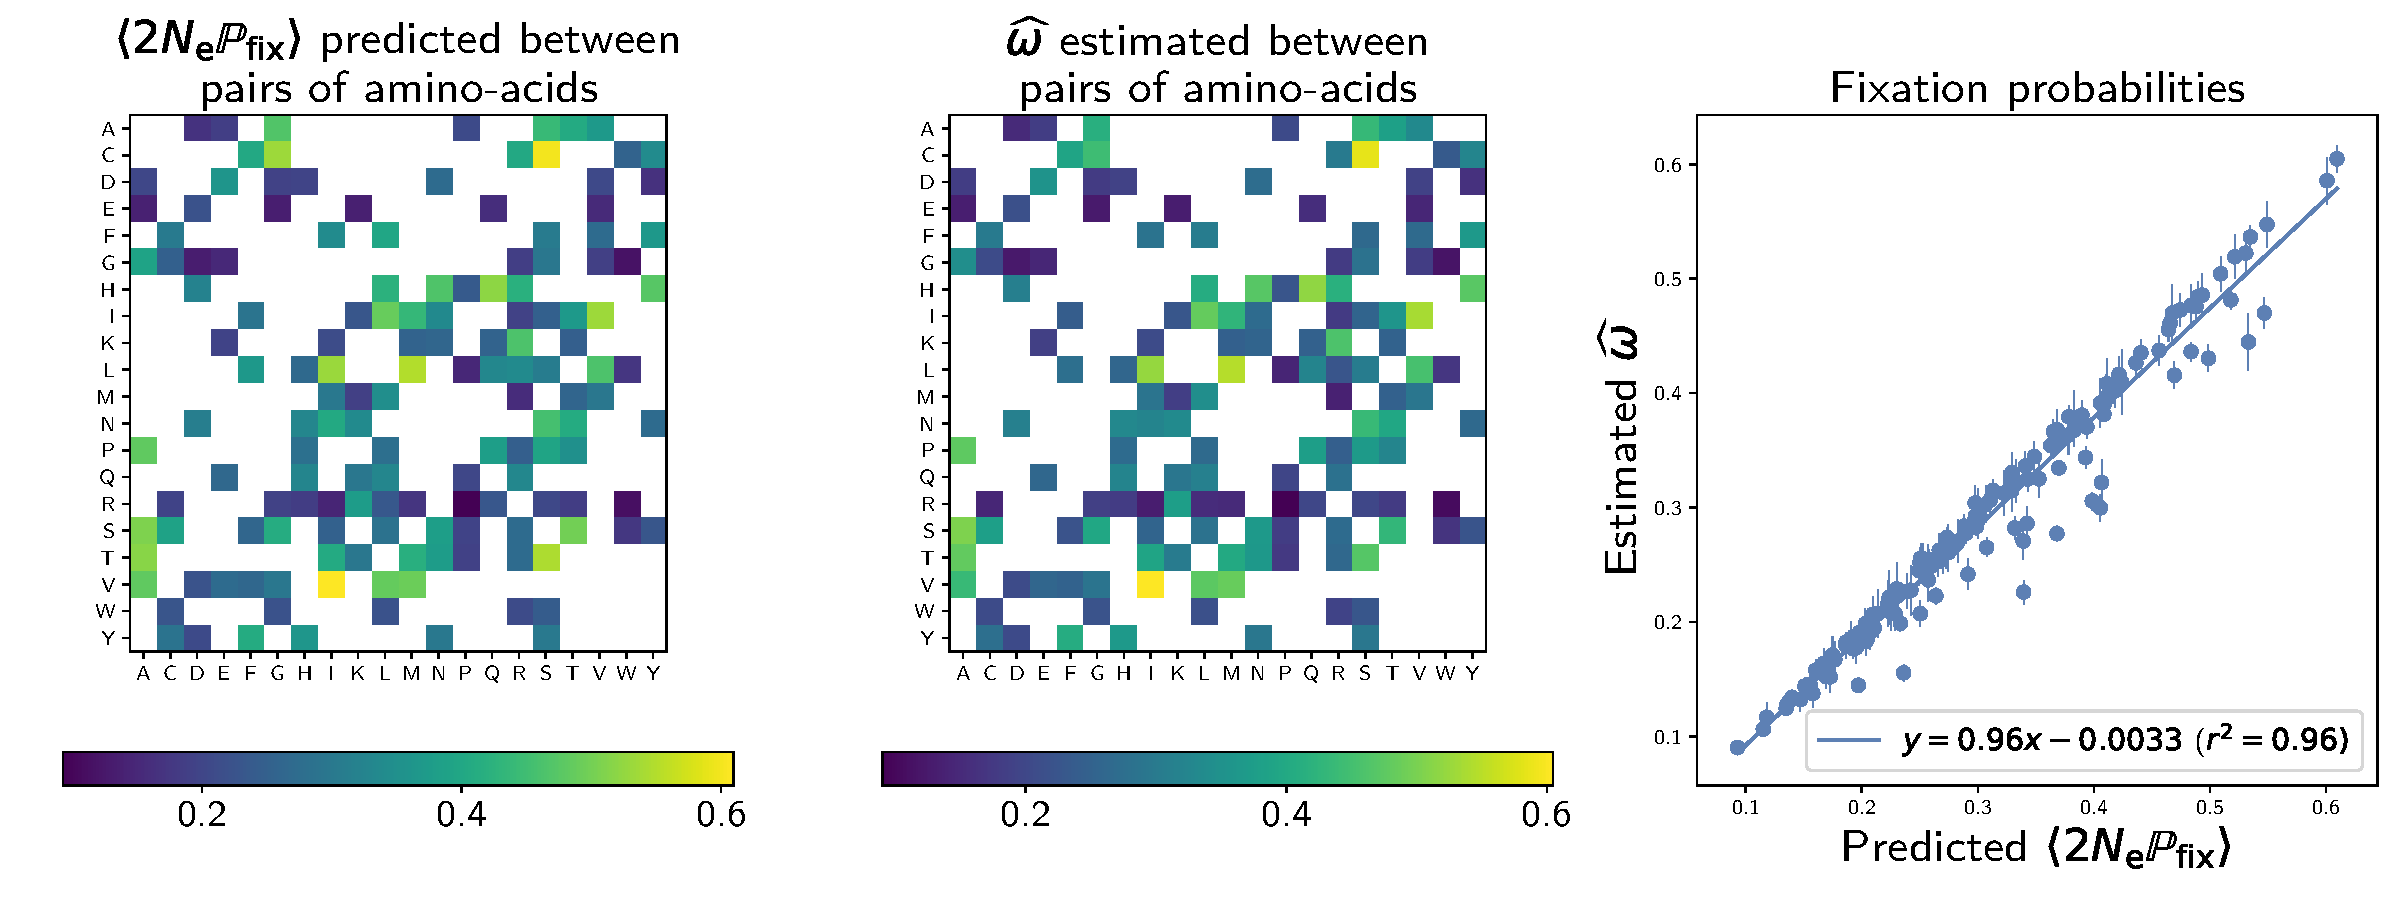
\includegraphics[width=\linewidth, page=1]{inference_simulations/omega_MF}
 \caption[Estimation of fixation probability]{
 Theoretical and estimated values of $\omega$ between pairs of amino-acids.
 The gene-wide prediction of the mean scaled fixation probability $\avgpfixAA$ between any pairs of amino-acids ($\aaSource, \aaTarget$) is given by equation~\ref{eq:omega_pairs_predicted}, as a function of the underlying site-specific fitness profiles and the mutation matrix.
 The mean estimated values of $\widehat{\omega}_{\aaSource, \aaTarget}$ are obtained by fitting the mean-field model (equation~\ref{eq:codon-mean-field}) onto the generated simulated alignment at the primate scale (61 primates taxa, 4980 codon sites, 100 repeats). The 95\% confidence for the mean value is represented with vertical bars.
 Given a large enough alignment, the mean-field estimation of pairwise fixation probabilities converge toward the predicted values.
 }
 \label{fig:omega-inference}
\end{figure}

We would like to derive a codon model that would be more accurate than the Muse \& Gaut model, but that would still be site-homogeneous.
However, the true process is site-specific.
The link between the two can be formalized by projecting the site-specific processes onto a gene-wise process, using what can be seen as a mean-field approximation.
The gene-wise process obtained by this procedure is expressed in terms of mutation rates and mean scaled fixation probabilities.
Finally, the mean scaled fixation probabilities can be identified with the $\omega$-tensor.

Specifically, at each site $\site$, the true codon process is:
\begin{equation}
 \begin{dcases}
 \submatrix_{\itoj}\siteexp & = 0 \text{ if codons $\ci$ and $\cj$ are more than one mutation away,} \\
 \submatrix_{\itoj}\siteexp & = \mutmatrix_{\nucitoj} \text{ if codons $\ci$ and $\cj$ are {synonymous},} \\
 \submatrix_{\itoj}\siteexp & = \mutmatrix_{\nucitoj} \Pfix\siteexp(\itoj) \text{ if codons $\ci$ and $\cj$ are non-synonymous}.
 \end{dcases}
 \label{eq:codon-site-processs}
\end{equation}
Where $\Pfix\siteexp(\itoj)$ is the scaled fixation probability of codon $\cj$ against codon $\ci$, at site $\site$.
At equilibrium of the process, averaging over sites gives the mean-field gene-level process:
\begin{equation}
 \begin{dcases}
 \left\langle \submatrix_{\itoj} \right\rangle & = 0 \text{ if codons $\ci$ and $\cj$ are more than one mutation away,} \\
 \left\langle \submatrix_{\itoj} \right\rangle & = \mutmatrix_{\nucitoj} \text{ if codons $\ci$ and $\cj$ are {synonymous},} \\
 \left\langle \submatrix_{\itoj} \right\rangle & = \mutmatrix_{\nucitoj} \left\langle \Pfix (\itoj) \right\rangle \text{ if codons $\ci$ and $\cj$ are non-synonymous}.
 \end{dcases}
 \label{eq:codon-avg-process}
\end{equation}
However, because selection between codons reduces to selection between pairs of amino-acids, $\left\langle \Pfix (\itoj) \right\rangle$ only depends on the amino-acids encoded by $\ci$ and $\cj$ (section~\ref{subsec:mean-field-derivation} in methods).
Thus, by identification, the inference model should be parameterized by a set of $\omega$ values for all pairs of amino acids, denoted $\omega_{\aaSource, \aaTarget}$.
For $20$ amino acids, the total number of pairs of amino acids is $190$, hence $380$ parameters by counting in both directions.
However, because of the structure of the genetic code, there are $75$ pairs that are one nucleotide away, since some amino acids are not directly accessible through a single {non-synonymous} mutation.
As a result, the number of parameters necessary to determine all non-zero entries of the tenser ($\omega_{\aaSource, \aaTarget}$) in both directions is $150$.
Finally, under the assumption of a reversible process, the number of parameters can be reduced to $75$ symmetric exchangeabilities ($\AAexchan_{\aaSource, \aaTarget}$) and $20$ stationary effects ($\AAequi_{\aaSource}$):
\begin{equation}
 \omega_{\aaSource, \aaTarget} = \AAequi_{\aaTarget} \AAexchan_{\aaSource, \aaTarget}\text{, where } \AAexchan_{\aaSource, \aaTarget} = \AAexchan_{\aaTarget, \aaSource}.\label{eq:omega-reversible}
\end{equation}

Altogether, the {substitution} rates between codons $\submatrix_{\itoj}$ are defined as:
\begin{equation}
 \begin{dcases}
 \submatrix_{\itoj} & = 0 \text{ if codons $\ci$ and $\cj$ are non neighbors}, \\
 \submatrix_{\itoj} & = \mutmatrix_{\nucitoj} \text{ if codons $\ci$ and $\cj$ are {synonymous},}, \\
 \submatrix_{\itoj} & = \mutmatrix_{\nucitoj} \omega_{\aai, \aaj} \text{ if codons $\ci$ and $\cj$ are non-synonymous},
 \end{dcases}
 \label{eq:codon-mean-field}
\end{equation}
where $\aai$ is the amino acid encoded by codon $\ci$ and $\omega_{\aaSource, \aaTarget}$ is given by equation~\ref{eq:omega-reversible}.

This mean-field ({MF}) model is fitted by maximum {likelihood}, giving an estimate for its parameters, $\widehat{\Mutmatrix}$, $\widehat{\AAExchan}$ and $\widehat{\AAEqui}$.
Then, from the estimate of the {GTR} nucleotide matrix ($\widehat{\Mutmatrix}$), a mutation bias $\widehat{\lambda}_{\text{{MF}}}$ can be estimated as previously (equation~\ref{eq:lambda-R} above).

As shown in the right panel of figure~\ref{fig:mut-bias-inference}, $\widehat{\lambda}_{\text{{MF}}}$ under the {MF} model provides an accurate estimate of the true mutational.
In other words, the {MF} model can tease out the observed $\atgc$ bias of the alignment and the underlying mutational bias.

The mean scaled fixation probability of {non-synonymous} mutations $\avgpfix$ can also be computed.
It is now a compound parameter, expressed as a function of $\widehat{\Mutmatrix}$, $\widehat{\AAExchan}$ and $\widehat{\AAEqui}$ (see section~\ref{sec:mut-bias-mean-field-omega}).
Under this model, $\avgpfix$ is close to the true mean scaled fixation probability $\avgpfix$ computed during the simulation, with a precision of 96.9\% (61 primates taxa, 4980 codon sites, 100 repeats).
Moreover, as shown in figure~\ref{fig:omega-inference}, the estimated rates $\widehat{\omega}_{\aaSource, \aaTarget}$ between pairs of amino acids is congruent with the predicted mean scaled fixation probability computed analytically as a function of the underlying site-specific fitness profiles and the mutation matrix as in equation~\ref{eq:omega_pairs_predicted}.

\subsection{Estimation on empirical sequence data}
\label{subsec:estimation-of-empirical-sequence-data}

The two alternative models of inference just considered, namely the classical Muse \& Gaut ({MG}) and the mean-field ({MF}) codon models, were then applied to empirical protein-coding sequence alignments.
Several examples were analysed: the nucleoprotein in \textit{Influenza Virus} (as human host) assembled in \citet{Bloom2017}, the $\beta$-lactamase in \textit{bacteria} gathered in \citet{Bloom2014}, as well as orthologous gene in primates extracted from OrthoMam database~\citep{Scornavacca2019} or from \citet{Perelman2011} as shown in table~\ref{tab:mut-bias-estimation}.

For alignment globally biased toward AT (nucleoprotein and AT-rich concatenate in primates), similarly to what was observed in the simulation experiments presented above, the mutational bias estimates under the two codon models are greater than the observed nucleotide bias (i.e.~$1 < \atgc < \widehat{\lambda}$).
This effect is, as previously, probably due to selection at the level of amino acids, partially opposing the mutational bias.
More importantly, the mutational bias estimated by the {MF} model is more extreme than the {MG} estimate (i.e.~$1 < \widehat{\lambda}_{\text{{MG}}} < \widehat{\lambda}_{\text{{MF}}}$).
These examples behaves identically to the observations made with simulated alignments, where, compared to {MG}, the {MF} model estimates a stronger mutational bias, which was also closer to the real value.
Thus, a reasonable interpretation is that {MG} is also underestimating the underlying mutational bias in the present case, and that the estimate of the {MF} model is more accurate.

Concerning selection, the estimated mean scaled fixation probability of {non-synonymous} mutations, is similarly estimated in the {MF} and {MG} models ($\avgpfix \simeq \widehat{\omega}$).
Additionally, in the {MF} model, $\avgpfix$ can be restricted to mutations from weak nucleotides (AT) to strong (GC), or vice versa (see section~\ref{sec:mut-bias-mean-field-omega}).
We observe that under a mutational bias favouring AT (i.e.~$\lambda > 1$), the mean fixation probability of {non-synonymous} mutations is higher toward GC than toward AT, $\avgpfixATtoGC > \avgpfixGCtoAT$, as expected under a AT-biased mutation process.

Reciprocally, for alignment globally biased toward GC ($\beta$-lactamase), the estimated mutation bias is stronger (toward GC) than the alignment bias (i.e.~$\widehat{\lambda}_{\text{{MF}}} < \atgc < 1$).
Curiously, in $\beta$-lactamase, the {MG} model estimates a weaker underlying mutational bias than the observed bias (i.e.~$ \atgc < \widehat{\lambda}_{\text{{MG}}} < 1$).
Concerning selection, we observe that the fixation probability of {non-synonymous} mutations is higher on average toward AT than toward GC, $\avgpfixGCtoAT > \avgpfixATtoGC$, as expected under a GC-biased mutation process.

The results obtained on empirical data are globally in agreement with the observations gathered from the simulation experiments, namely that the presence of a mutational bias results in a selection differential, taking the form of a slightly higher mean fixation probability of {non-synonymous} mutations opposing the mutational bias.
Moreover, by setting $\AAEqui = \vecOne$ and $\AAExchan = \omega \times \vecOne$ in our mean-field model, we retrieve the nested Muse \& Gaut model, hence, both models are directly comparable.
The empirical fit to the data between the nested models, using AIC and Likelihood ratio test~\citep{Posada2004}, always favors the MF model compared to the MG model.
Altogether, our {MF} model is favored by empirical dataset, and simultaneously estimates more extreme (and probably more accurate) mutational biases compared to the {MG} model.

\begin{table}[h]
 \centering
 \noindent\adjustbox{max width=\textwidth}{%
  \begin{tabu}{l||c|c|c|c|c|c|c|c|c|c|}
   \toprule
   {} & $\beta$-Lactamase & Nucleoprotein & Primates AT-rich & Primates & Hominoidea & Cercopithecoidea & Platyrrhini & Simiiformes & Catarrhini \\
   \midrule
   \textbf{Dataset} & \citeauthor{Bloom2014} & \citeauthor{Bloom2017} & \citeauthor{Scornavacca2019} & \citeauthor{Perelman2011} & \citeauthor{Perelman2011} & \citeauthor{Perelman2011} & \citeauthor{Perelman2011} & \citeauthor{Perelman2011} & \citeauthor{Perelman2011} \\
   \textbf{Number of taxa} & \large{85} & \large{180} & \large{22} & \large{61} & \large{7} & \large{18} & \large{15} & \large{40} & \large{25} \\
   \textbf{Number of sites} & \large{263} & \large{498} & \large{4877} & \large{5300} & \large{5300} & \large{5300} & \large{5300} & \large{5300} & \large{5300} \\
   \textbf{$\atgc$} & \large{0.792} & \large{1.154} & \large{2.028} & \large{1.075} & \large{1.098} & \large{1.096} & \large{1.098} & \large{1.097} & \large{1.097} \\
   \textbf{$\atgc$ at first coding position} & \large{0.583} & \large{1.057} & \large{1.303} & \large{0.996} & \large{1.008} & \large{1.000} & \large{1.009} & \large{1.005} & \large{1.002} \\
   \textbf{$\atgc$ at second coding position} & \large{1.177} & \large{1.221} & \large{2.541} & \large{1.426} & \large{1.439} & \large{1.440} & \large{1.444} & \large{1.441} & \large{1.440} \\
   \textbf{$\atgc$ at third coding position} & \large{0.714} & \large{1.192} & \large{2.648} & \large{0.878} & \large{0.916} & \large{0.918} & \large{0.913} & \large{0.916} & \large{0.918} \\
   \textbf{MG mutational bias ($\widehat{\lambda}_{\text{{MG}}}$)} & \large{0.853} & \large{1.447} & \large{2.073} & \large{1.139} & \large{1.162} & \large{1.177} & \large{1.187} & \large{1.205} & \large{1.178} \\
   \textbf{MF mutational bias ($\widehat{\lambda}_{\text{{MF}}}$)} & \large{0.690} & \large{1.748} & \large{2.419} & \large{1.022} & \large{0.995} & \large{1.024} & \large{1.057} & \large{1.108} & \large{1.038} \\
   \textbf{MG }$\bm{\widehat{\omega}}$ & \large{0.332} & \large{0.114} & \large{0.526} & \large{0.272} & \large{0.367} & \large{0.316} & \large{0.333} & \large{0.325} & \large{0.328} \\
   \textbf{MF }$\bm{\avgpfix}$ & \large{0.336} & \large{0.116} &0.525 & \large{0.272} & \large{0.380} & \large{0.318} & \large{0.343} & \large{0.332} & \large{0.334} \\
   \textbf{MF }$\bm{\avgpfixATtoGC}$ & \large{0.297} & \large{0.141} & \large{0.594} & \large{0.254} & \large{0.325} & \large{0.292} & \large{0.302} & \large{0.303} & \large{0.303} \\
   \textbf{MF }$\bm{\avgpfixATtoGC}$ & \large{0.412} & \large{0.092} & \large{0.487} & \large{0.308} & \large{0.410} & \large{0.363} & \large{0.362} & \large{0.347} & \large{0.369} \\
   \textbf{$\bm{\Delta}$AIC} & \large{37.6} & \large{165.2} & \large{1527.0} & \large{1091.0} & \large{371.6} & \large{359.8} & \large{487.9} & \large{586.2} & \large{403.5} \\
   \textbf{$\bm{p\left( \chi_{\text{df=}93}^2 > \text{LRT}\right)}$} & \large{9.2$\times 10^{-13}$} & \large{1.2$\times 10^{-31}$} & \large{3.9$\times 10^{-296}$} & \large{2.9$\times 10^{-207}$} & \large{2.2$\times 10^{-67}$} & \large{3.1$\times 10^{-65}$} & \large{6.6$\times 10^{-89}$} & \large{1.4$\times 10^{-107}$} & \large{3.3$\times 10^{-73}$} \\
   \bottomrule
  \end{tabu}}
 \caption[Estimated parameters]{
  Estimated parameters of mutational bias ($\widehat{\lambda}$) from two models of inference, namely classical Muse \& Gaut ({MG}) and mean-field ({MF}).
  These models are applied to distinct datasets of protein-coding {DNA} alignments and concatenates of orthologous genes.
  By taking into account selection in multiple direction, {MF} models estimates a stronger mutational bias than the {MG} model, and has a statistically better fit than the MG model.
  For the {MG} model the mean scaled fixation probability of {non-synonymous} mutations ($\widehat{\omega}_{MF}$) can be obtained either from weak (AT) to strong nucleotides (GC), or vice versa.
  The fixation probability of {non-synonymous} mutations is opposed to the underlying mutational bias, such that a skewed mutational process results in a skewed selection, justifying that they must be articulated together.
 }
 \label{tab:mut-bias-estimation}
\end{table}

\section{Discussion}\label{sec:discussion}

In protein-coding {DNA} sequences, the nucleic composition results from a subtle interplay between mutation at the nucleic level and selection at the protein level.
As a result, the observed nucleotide bias in the alignment is different from the underlying mutational bias.

However, current parametric codon models are inherently misspecified and, for that reason, are unable to tease apart these opposing effects of mutation and selection correctly.
As a result, they don't estimate the mutational process reliably.

In this work we sought to find the simplest parametric codon model able to correctly tease apart mutation rates on one hand, and net mean fixation probabilities on the other hand, and this, without having to explicitly model the underlying fitness landscape.
In order to derive a codon model along those lines, our strategy is to first assume an underlying microscopic model of sequence evolution (here, a mutation-selection model based on a site-specific, time-independent fitness landscape).
Then, we derive the gene-wise mean fixation probabilities between all pairs of codons, implied by the underlying microscopic process.
Finally, we observe that this mean-field process should in fact invoke as many distinct $\omega$ parameters as there are pairs of amino acids that are nearest neighbours in the genetic code.
There are reversibility conditions, reducing the dimensionality and allowing for a GTR-like parameterization of this tensor ($95$ parameters for selection).

Inferring parameters on simulated alignments, we show that the model derived using this mean-field argument correctly estimates the underlying mutational bias and selective pressure.
Applied to empirical alignments, we also observe that there is a selection differential opposing the mutational bias.

This work first points to a fundamental property of natural genetic sequences, namely that they are not optimized but are the result of an equilibrium between forces.
In the specific case highlighted in this work, mutational bias at the nucleotide-level results in suboptimal amino-acid being overrepresented in the sequence.
This was pointed out previously~\citep{Singer2000}, although never directly formalized in phylogenetic codon model.

One important consequence of this tradeoff between mutation and selection at equilibrium is that the observed higher mean fixation probability toward GC is mimicking the effect of biased gene conversion toward GC ({gBGC}), although unlike {gBGC}, the phenomenon described here corresponds to a genuine selective effect.
Although we did not explore the consequences of this at the level of intra-specific polymorphism, the selection differential uncovered here also implies that the distribution of fitness effects is not the same in the two directions, either toward AT or toward GC.
Specifically, in the presence of an AT-biased mutation process, the {non-synonymous} GC polymorphisms are expected to segregate at higher frequencies, compared to {non-synonymous} AT polymorphisms.

These observations have some practical implications: for instance, experiments observing a fixation (or segregation) bias toward GC at the {non-synonymous} level must also rule out that this fixation bias is not a simple consequence of the mutation-selection balance.
More generally, our observations and modelling principles offer a useful preliminary basis to better understand how mutation and selection will work together with biased gene conversion ({gBGC}), and therefore will help better understand how {gBGC} will impact both nucleotide composition and $\dnds$.
It is worth mentioning that in our result, we focused on the fixation probability from AT to GC, $\avgpfixATtoGC$, because of the relationship to {gBGC}.
However, in practice, the same analysis and methods can be applied to any subset of nucleotides or codons.

Our mean-field parametric model uses gene-level parameters (in the form of a tensor) that is meant to capture the mean scaled fixation probabilities.
This derivation, and its validation on simulated data, shows that, even though the underlying selective landscape is site-specific, a gene-level approximation can nonetheless accurately disentangles mutation and selection.
As a result, this study demonstrates that phenomenological models derived out of mechanistic models are more compact (i.e.~not site-specific), and in certain cases are sufficient to extract the relevant parameters.

The methodology proposed here for deriving inference models consists in proceeding in two steps, first assuming an underlying mechanistic model of sequence evolution, parameterized by variables that are derived from first principles (fitness landscape, mutations rates, $\hdots$).
Subsequently, the phenomenological inference model is obtained by matching its parameters (here, the entries of the $\omega$ tensor) with the aggregate parameters derived from the application of the mean-field procedure to the mechanistic model.
Altogether, we believe that the approach used here could be applied more generally: inference models can be phenomenological in practice, but should nonetheless be derived from an underlying mechanistic model, so as to correctly formalize the interplay between mutation, selection, drift and other evolutionary forces.

Finally, this work is still preliminary since the mean-field model should be tested against a more diverse range of empirical data, in terms of phylogenetic depth, strength of selection, and {codon usage bias} to assert the validity of our empirical results.
In addition, several other codon models~\citep{Rodrigue2008a,KosakovskyPond2020} should be included in a broader comparison of the accuracy of the estimation of the underlying mutational bias and strength of selection on protein-coding {DNA} sequences.

\section{Materials \& Methods}

\subsection{Simulation model}
\label{sec:mut-bias-simu}
We seek to simulate the evolution of protein-coding sequences along a specie tree.
Starting with one sequence at the root of the tree, the sequences evolve independently along the different branches of the tree by point {substitutions}, until they reach the leaves.
At the end of the simulation, we get one sequence for each leaf of the tree, meaning one sequence per species.
The {substitution} is modelled using the origination-fixation approximation, i.e.~substitution rates are the product of the mutation rate at the nucleotide level, and fixation probabilities, based on selection at the amino-acid level.

The mutation process is assumed homogeneous across sites.
On the other hand, selection is assumed to be varying along the sequence.
During the simulation, given the current sequence, the {substitution} rates toward all possible mutants (one nucleotide change) are computed and the next {substitution} event is drawn randomly based on Gillespie's algorithm~\citep{Gillespie1977}.

\subsection{Mutational bias at the nucleotide level}
\label{sec:mut-bias-mut-matrix}
The mutation rate between nucleotides is always proportional to $\mu$.
Moreover, mutations from any nucleotide to another weak nucleotide is increased by the factor $\lambda$ compared with mutations to another strong nucleotide.
The mutation rate matrix is thus:
\begin{equation}
 \label{nucMatrix}
 \Mutmatrix =
 \begin{blockarray}{ccccc}
 & A & C & G & T \\
 \begin{block}{c(cccc)}
 A & {-\mu(2 + \lambda)} & {\mu} & {\mu} & {\mu \lambda} \\
 C & {\mu \lambda} & {-\mu(1 + 2\lambda)} & {\mu} & {\mu \lambda} \\
 G & {\mu \lambda} & {\mu} & {-\mu(1 + 2\lambda)} & {\mu \lambda} \\
 T & {\mu \lambda} & {\mu} & {\mu} & {-\mu(2 + \lambda)} \\
 \end{block}
 \end{blockarray}
\end{equation}
Which has the following stationary distribution:
\begin{align}
 \Mutequi \Mutmatrix & = \vecOne, \\
 \iff \Mutequi & = \left( \dfrac{\lambda}{2+2\lambda}, \dfrac{1}{2+2\lambda}, \dfrac{1}{2+2\lambda}, \dfrac{\lambda}{2+2\lambda} \right).
 \label{nucStationarity}
\end{align}
As a result, the ratio of weak over strong nucleotide frequencies at stationarity is equal to $\lambda$:
\begin{align}
 \label{lambda}
 \dfrac{ \mutequi_A + \mutequi_T }{ \mutequi_C + \mutequi_G }
 & = \dfrac{ \lambda ( 2 + 2 \lambda)^{-1} + \lambda ( 2 + 2 \lambda)^{-1}}{ ( 2 + 2 \lambda)^{-1} + ( 2 + 2 \lambda)^{-1}}, \ \text{from eq.~\ref{nucStationarity},}\\
 & = \lambda.
\end{align}
$\mu$ is constrained such the expected flow (- $\sum_{a} \mutequi_a \mutmatrix_{a, a} $) of mutation equals to $1$.

\subsection{Selection at the amino-acid level}
\label{sec:mut-bias-aa-selection}

The {substitution} rate is considered null between any two codons differing by more than one nucleotide.
Otherwise, the mutation rate between a pair of codons is given by the mutation rate of the underlying single nucleotide change.
Selection is modelled at the amino-acid level, i.e.~we assume that all codons encoding for one particular amino acid are selectively {neutral}.

To take into account the heterogeneity of selection between different sites of the protein, we assume that each site $\site$ of the sequence is independently evolving under a site-specific fitness landscape, characterized by a 20-dimensional frequency vector of scaled (Wrightian) fitness parameters $\Profile\siteexp = \{ \profile\siteexp_{\aminoacid},\ 1 \leq \aminoacid \leq 20 \}$.
The fitness vectors $\Profile\siteexp$ used in this study are extracted from \citet{Bloom2017}, which were experimentally determined by deep mutational scanning for 498 codon sites of the nucleoprotein in \textit{Influenza Virus} strains (as human host).
For each {codon} site $\site$ of our simulation, we assign randomly one the 498 fitness profile (sampling with replacement) experimentally determined, which altogether determines the (Wrigthian) fitness vectors across sites.
The malthusian fitness (or log-fitness) of amino acid $\aminoacid$, denoted $\scaledfit\siteexp_{\aminoacid}$, is scaled by the relative effective population size ($\Ner$) accordingly:
\begin{equation}
 \scaledfit\siteexp_{\aminoacid} = \Ner \ln \left( \profile\siteexp_{\aminoacid} \right),\ \Setsite, \ \SetAa
\end{equation}
At site $\site$, the {substitution} rate between {non-synonymous} codons $\ci$ and $\cj$ is given by the product of the mutation rate and the probability of fixation:
\begin{equation}
 \submatrix_{\itoj}\siteexp = \mutmatrix_{\nucitoj} \dfrac{\Fitj\siteexp - \Fiti\siteexp}{1 - \e^{\Fiti\siteexp - \Fitj\siteexp} } \label{eq:codonsubrates}
\end{equation}
where $\aai$ denotes the amino-acid encoded by codon $\ci$.
At the root of the tree, for each site $\site$, the sequence is drawn from the stationary distribution of the process specified by $\Subequi\siteexp$, which is given by:
\begin{align}
 \subequi_{\ci}\siteexp & = \mathcal{Z}\siteexp \left[\prod\limits_{k \in \{ 1, 2, 3 \}} \mutequi_{\ci[k]}\right] \e^{\Fiti\siteexp},
 \label{codonStationarity}
\end{align}
where $\ci[k]$ denotes the nucleotide at position $k \in \{ 1, 2, 3 \}$ of codon $\ci$, and $\mathcal{Z}\siteexp $ is the normalizing constant at site $\site$:
\begin{align}
 \mathcal{Z}\siteexp = \left( \sum\limits_{\cj=1}^{61} \left[\prod\limits_{k \in \{ 1, 2, 3 \}} \mutequi_{\cj[k]}\right] \e^{\Fitj\siteexp} \right)^{-1}
\end{align}
The {substitution} process is reversible and fulfils detailed balance conditions at each site $\site$ and between each pair of codons ($\ci$, $\cj$):
\begin{align}
 \subequi_{\ci}\siteexp \submatrix_{\itoj}\siteexp = \subequi_{\cj}\siteexp \submatrix_{\cj, \ci}\siteexp
 \label{codonSubBalance}
\end{align}

Of note, by modelling fitness at the amino-acid level, we assume that all codons encoding for one particular amino acid are selectively {neutral}.
In addition, in this modelling framework, the genetic code is of particular importance since the number of codons encoding for a particular amino acid varies greatly.
As an example, tryptophan is encoded by one codon, while leucine is encoded by 6 codons.
Intuitively, this variation makes the mutation bias more pronounced among codons encoding for the same amino acid, since there are more mutations possible that are selectively {neutral} (i.e. synonymous).
On the other hand, the mutation bias is more constrained if the amino acid is encoded by few codons.

\subsection{Mean scaled fixation probability}
\label{subsec:fixation-bias}
The sequence at time $t$ is denoted $\Seqi(t)$ and the codon present at site $\site$ is denoted $\Seqi_{\site}(t)$.
For a given sequence, the mean scaled fixation probability over mutations away from $\Seqi(t)$, weighted by their probability of occurrence, is given by the ratio:
\begin{align}
 \avgpfixtime & = \dfrac{ \sum\limits\sumSetsite \sum\limits_{\cj \in \NonSynNeighbors \left ( \Seqi_{\site}(t) \right)} Q_{\Seqi_{\site}(t) \to \cj}}{ \sum\limits\sumSetsite \sum\limits_{\cj \in \NonSynNeighbors \left ( \Seqi_{\site}(t) \right)} \mu_{\Seqi_{\site}(t) \to \cj}},
\end{align}
where $\setNonSynNeighbors$ is the set of {non-synonymous} codons neighbours of codon $\ci$ and $\submatrix_{\itoj}\siteexp$ are defined as in equation~\ref{eq:codonsubrates}.
Averaged over all branches of the tree, the mean scaled fixation probability is :
\begin{align}
 \avgpfix & = \int_{t} \avgpfixtime \der t,
\end{align}
where the integral is taken over all branches of the tree, while the integrand $\avgpfixtime$ is a piece-wise function changing after every point {substitution} event.
The mean scaled fixation probability from weak (AT) to strong (GC) nucleotides, denoted $\avgpfixATtoGC$, is obtained similarly by restricting the sums (in the numerator and the denominator) from weak to strong mutations.
A similar computation can be done from strong to weak.

\subsection{Derivation of mean-field model}
\label{subsec:mean-field-derivation}
The mean-field codon model $\left\langle \Submatrix \right\rangle$ is defined such that $\left\langle \submatrix_{\itoj} \right\rangle$ is the average rate of {substitution} to codon $\cj$, conditional on currently being on codon $\ci$, the average being taken across sites.
Importantly, sites differ in their probability of being currently in state $\ci$.
The average should therefore be weighted by this probability.

Assuming an underlying site-specific mutation-selection process at equilibrium, given we know that a mutation is from codon $\ci$, the probability that this mutation is occuring at site $\site$ is:
\begin{align}
 \proba (\site \mid \ci) = \dfrac{ \subequi_{\ci}\siteexp }{\sum\limits\sumSetsite \subequi_{\ci}\siteexp }
\end{align}
The site-averaged (mean-field) {substitution} rate from codon $\ci$ to $\cj$ is as result given as:
\begin{align}
 \left\langle \submatrix_{\itoj} \right\rangle = \sum\limits\sumSetsite \proba (\site \mid \ci) \submatrix_{\itoj}
\end{align}
If codon $\ci$ and codon $\cj$ are {synonymous}, this equation simplifies to the underlying mutation rate $\mutmatrix_{\nucitoj}$.
Otherwise, if codon $\ci$ and codon $\cj$ are {non-synonymous}, the mean-field {substitution} rate is:
\begin{align}
 \left\langle \submatrix_{\itoj} \right\rangle & = \left\langle \mutmatrix_{\nucitoj} \Pfix (\itoj) \right\rangle, \\
 & = \mutmatrix_{\nucitoj} \left\langle \Pfix (\itoj) \right\rangle, \\
 & = \mutmatrix_{\nucitoj} \dfrac{ \sum\limits\sumSetsite \subequi_{\ci}\siteexp \dfrac{\Fitj\siteexp - \Fiti\siteexp}{1 - \e^{\Fiti\siteexp - \Fitj\siteexp}} }{ \sum\limits\sumSetsite \subequi_{\ci}\siteexp }, \\
 & = \mutmatrix_{\nucitoj} \dfrac{ \sum\limits\sumSetsite \mathcal{Z}\siteexp \dfrac{\Fitj\siteexp - \Fiti\siteexp}{ \e^{-\Fiti\siteexp} - \e^{ - \Fitj\siteexp}} }{ \sum\limits\sumSetsite \mathcal{Z}\siteexp \e^{\Fiti\siteexp} }
\end{align}
As a result, $\left\langle \Pfix (\itoj) \right\rangle$ is dependent on the source and target codon solely through the source amino acid ($\aaSource$) and target amino acid ($\aaTarget$), hence the parameter $\omega_{\aaSource, \aaTarget}$ identifies with the average fixation probability $\avgpfixAA$:
\begin{equation}
 \label{eq:omega_pairs_predicted} \avgpfixAA = \dfrac{ \sum\limits\sumSetsite \mathcal{Z}\siteexp \dfrac{\FitaaTarget\siteexp - \FitaaSource\siteexp}{ \e^{-\FitaaSource\siteexp} - \e^{ - \FitaaTarget\siteexp}} }{ \sum\limits\sumSetsite \mathcal{Z}\siteexp \e^{\FitaaSource\siteexp} }.
\end{equation}

\subsection{Mean scaled fixation probability $\avgpfix$ under the mean-field model}
\label{sec:mut-bias-mean-field-omega}
The mean-field model is parameterized by a {GTR} mutation matrix $\Mutmatrix(\Mutequi, \Exchan)$ and the selection coefficient $\UniDimArray{\omega}(\AAExchan, \AAEqui)$.
As a result, the mean scaled fixation probability of {non-synonymous} mutations is:
\begin{align}
 \avgpfix & = \dfrac{ \sum\limits\sumOverCodons \subequi_{\ci} \sum\limits_{\cj \in \setNonSynNeighbors} Q_{\itoj}}{ \sum\limits\sumOverCodons \subequi_{\ci} \sum\limits_{\cj \in \setNonSynNeighbors} \mu_{\itoj}}, \\
 & = \dfrac{ \sum\limits\sumOverCodons \left[\prod\limits_{k \in \{ 1, 2, 3 \}} \mutequi_{\ci[k]}\right] \AAequi_{\aai} \sum\limits_{\cj \in \setNonSynNeighbors} \mutmatrix_{\nucitoj} \AAequi_{\aaj} \AAexchan_{\aai, \aaj} }{\sum\limits\sumOverCodons \left[\prod\limits_{k \in \{ 1, 2, 3 \}} \mutequi_{\ci[k]}\right] \AAequi_{\aai} \sum\limits_{\cj \in \setNonSynNeighbors} \mutmatrix_{\nucitoj}},
\end{align}
where $\ci[k]$ denotes the nucleotide at position $k \in \{ 1, 2, 3 \}$ of codon $i$.

Similarly, the mean scaled fixation probability from weak (AT) to strong (GC) nucleotides denoted $\avgpfixATtoGC$ is obtained similarly by restricting the sums (in the numerator and the denominator) to one nucleotide mutations only from weak to strong.
Conversely, by restricting the sum from strong (GC) to weak (AT), we obtain $\avgpfixGCtoAT$.

\subsection{Inference method with \texttt{Hyphy}}
\label{subsec:inference-method-with-hyphy}

Maximum {likelihood} estimation has been performed with the software \texttt{Hyphy}~\citep{Pond2005}.
The \texttt{Python} scripts generating the \texttt{Hyphy} batch files (for both Muse \& Gaut and mean-field), as well as scripts necessary to replicate the experiments are available at \url{https://github.com/ThibaultLatrille/NucleotideBias}.

\section{Data availability}
The data underlying this article are available in Github, at \url{https://github.com/ThibaultLatrille/NucleotideBias}, as well as scripts and instructions necessary to reproduce the simulated and empirical experiments.
The simulators written in \texttt{C++} are available at \url{https://github.com/ThibaultLatrille/SimuEvol}.
Supplementary materials describing additional analysis are available online.

\section{Author contributions}
TL gathered and formatted the data, developed the new models in \texttt{SimuEvol} and conducted all analyses, in the context of a PhD work (Ecole Normale Superieure de Lyon).
TL and NL both contributed to the writing of the manuscript.

\section{Acknowledgements}
We gratefully acknowledge the help of Laurent Gueguen, Laurent Duret, Christophe Douady and Benoit Nahbolz for their input on this work and their comments on the manuscript.
This work was performed using the computing facilities of the CC LBBE/PRABI.
Funding: French National Research Agency, Grant ANR-15-CE12-0010-01 / DASIRE.

\bibliographystyle{natbib}%%%%Bibliography style file
\bibliography{references, introduction}

\end{document}
